\documentclass{article}
% Auto-build test comment - SAVE THIS FILE TO TEST 

\usepackage{amsmath}
\usepackage{amssymb}    % For \checkmark, \texttimes, etc.
\usepackage[table]{xcolor} % For cell colors in table, and \yesmark, \nomark
\usepackage{array}      % For better column definitions in tables
\usepackage{booktabs}   % For professional-looking tables (\toprule, \midrule, \bottomrule)
\usepackage{caption}    % For table captions
\usepackage{graphicx}   % For \resizebox
\usepackage{makecell}   % For \makecell
\usepackage{enumitem}   % For custom enumerate labels
\usepackage[ruled,vlined]{algorithm2e} % For algorithm environment
% % \usepackage[inkscape]{svg} % Use inkscape for SVG to PDF conversion - COMMENTED OUT TO USE PNG - COMMENTED OUT TO USE PNG

\PassOptionsToPackage{table}{xcolor}
\usepackage{xcolor}  % loads xcolor with the table option

\usepackage{tcolorbox}
\newtcolorbox{primerbox}[1]{
  colback=blue!5!white,
  colframe=blue!75!black,
  fonttitle=\bfseries,
  title=#1,
  arc=2mm,
  boxsep=5pt,
  left=4pt,
  right=4pt,
  top=4pt,
  bottom=4pt
}

% Load inputenc and fontenc early
\usepackage[utf8]{inputenc}
\usepackage[T1]{fontenc}

\usepackage{edictive-arch}

\usepackage{float}

\usepackage{array}

\usepackage{siunitx}
% \sisetup{detect-all} % Deprecated
\sisetup{ % Modern siunitx font detection
    mode = match,
    propagate-math-font = true,
    reset-math-version = false,
    reset-text-family = false,
    reset-text-series = false,
    reset-text-shape = false,
    text-family-to-math = true,
    text-series-to-math = true
}

\usepackage{url,booktabs,amsfonts,nicefrac,microtype,xcolor}
\usepackage{hyperref}
\hypersetup{
    colorlinks=true,
    linkcolor=blue,
    filecolor=magenta,
    urlcolor=cyan,
    citecolor=blue, % Color for citations
}

% for table
\usepackage{array}
\usepackage{amssymb}    % \checkmark
\usepackage{graphicx}   % \resizebox
\usepackage{makecell}

% --- column types ---
\newcolumntype{L}[1]{>{\raggedright\arraybackslash}m{#1}}
\newcolumntype{C}[1]{>{\centering\arraybackslash}m{#1}}

% yes/no marks
\newcommand{\yesmark}{{\color{green!60!black}\checkmark}}
\newcommand{\nomark}{{\color{red}$\times$}}
\newcommand{\somewhatmark}{{\color{orange}$\approx$}}


% Define \ListOpsparams
\newcommand{\ListOpsparams}{(a maximum of 8 operations, a minimum arity of 4, and a maximum branching factor of 8 of the ListOps problem being narrativized)}

\usepackage{natbib}
\setcitestyle{authoryear,open={(},close={)}} % For (Author, Year) style citations

\title{Project Helios: Automating \\Predictive Signal Extraction}

\author{
  Alex Pan\\
  Founder, Edictive
}

\date{}  % omit the date

\begin{document}
\begingroup
\renewcommand\thefootnote{}
\endgroup
\maketitle
\begin{abstract}
  Large Language Models (LLMs) can improve time-series forecasting by incorporating textual context \citep{williams2025contextkeybenchmarkforecasting}, but the antecedent task of extracting predictive signals from unstructured text remains a critical bottleneck. We introduce Project Helios, a conceptual framework that operationalizes the hypothesis that this process can be automated by unifying synthetic data generation and automatic prompt optimization (APO). Helios's two-pillar architecture features (i) a minimal-configuration data generator using correlated sampling \citep{kowshik2024corrsynthcorrelatedsampling} and hard-case mining \citep{wu2024stragoharnessingstrategicguidance}, and (ii) a multi-objective prompt optimizer leveraging a novel hybrid algorithm, which we term Pareto-StraGo, that synthesizes concepts from Pareto-front optimization \citep{zhao2025pareto} and strategic guidance \citep{wu2024stragoharnessingstrategicguidance}. By tightly coupling these components, Helios provides a turnkey solution that transforms a high-level signal definition into an optimized, production-ready prompt, significantly accelerating the experimental cycle for signal engineering. This paper's contributions are: (1) the conceptual architecture, (2) a map of key design decisions, (3) a preliminary feasibility analysis, and (4) a research agenda, all motivated by the scaling imperatives of modern AI \citep{kaplan2020scalinglawsneurallanguage}.

\end{abstract}

\section{Introduction}
\label{sec:introduction}
The application of Large Language Models (LLMs) to time-series forecasting is increasingly prominent, driven by their unique ability to integrate rich, unstructured textual context into the forecasting process \citep{williams2025contextkeybenchmarkforecasting, ansari2024chronoslearninglanguagetime, jin2024timellmtimeseriesforecasting}. This contextual understanding allows LLMs to outperform traditional models in scenarios where external natural-language information is critical for accurate prediction. 

Yet the prerequisite step—extracting reliable predictive signals from vast, unstructured corpora such as sales calls, support tickets, or operational logs—remains labor-intensive and slow.  Conventional workflows rely on costly human annotation and bespoke model training, limiting hypothesis throughput and discouraging rapid experimentation.

We posit that the same instruction-following capacity that lets LLMs improve forecasts can also automate signal extraction when paired with two fast-moving ideas: synthetic data generation \citep{patel2024datadreamertoolsyntheticdata, kowshik2024corrsynthcorrelatedsampling} and automatic prompt optimization (APO) \citep{yang2024largelanguagemodelsoptimizers, zhao2025pareto}.  Project \textbf{Helios} is a conceptual framework that tightly couples these techniques in a closed loop: a zero-configuration generator fabricates rubric-aligned datasets, while a multi-objective optimizer searches for Pareto-efficient prompts; each component continuously red-teams the other, surfacing hard cases that sharpen the overall system.

This paper is a \emph{position piece}.  We present no empirical results and make no claims of experimental verification.  Our goal is to articulate a compelling architecture and research agenda that can attract community effort toward rigorous testing. We make the following novel contributions:\footnote{All contributions are architectural or analytical; empirical validation is left to future work.}

\begin{enumerate}[leftmargin=*,noitemsep]
  \item \textbf{Helios architecture}: a closed-loop design that unifies synthetic data generation with multi-objective APO for automated signal extraction.
  \item \textbf{Design-decision map}: a systematic treatment of nine key trade-offs (data blend, diversity vs.\ fidelity, etc.) to guide future implementers.
  \item \textbf{Feasibility analysis}: a cost–benefit and scalability discussion suggesting that Helios can cut iteration time from months to hours.
  \item \textbf{Research agenda}: open questions and practical milestones intended to catalyze empirical studies on the proposed approach.
\end{enumerate}

\section{From Manual Pipelines to Closed-Loop Automation}
\label{sec:evolution}
This section first traces the historical \emph{evolution} of textual-signal extraction, motivating the move from human-centric to data-centric pipelines.  It then states, in strict mathematical terms, the \emph{problem} that Project Helios sets out to solve.

\subsection{Stage 1: Human Annotation and Bespoke Models}
Domain experts hand-label thousands of examples, after which ML engineers train task-specific classifiers.  The process is costly, slow, and biased toward majority classes, yielding low macro-F1 on the minority signals that usually matter most (e.g., early-warning churn indicators) \citep{yu2023largelanguagemodelattributed}. This bias limits organizations' ability to efficiently explore diverse predictive signals, slowing hypothesis testing and model development.

\subsection{Stage 2: Partial Automation with Decoupled Components}
Two research threads emerged—but in isolation:

\begin{enumerate}
  \item \textbf{Synthetic data generation} cheapens labels via LLMs \citep{patel2024datadreamertoolsyntheticdata}, but without downstream feedback the generator is \emph{flying blind}. It often misses the `unknown-unknown' edge cases that decide real-world failure.
  \item \textbf{Automatic prompt optimization (APO)} tunes prompts for a \emph{fixed} evaluation set \citep{pryzant2023automaticpromptoptimizationgradient,lester2021powerscaleparameterefficientprompt}, yielding what we call \emph{vacuum optimization}: the prompt is optimal in sandbox yet brittle in production.
\end{enumerate}

With both paths locked to static data, they cannot reveal or balance multi-objective trade-offs (accuracy, latency, cost, safety). The situation echoes mode collapse in GANs, where a generator stagnates once the data supply stops evolving.

These shortcomings spotlight a broader shift toward \textit{data-centric AI}: holding the model fixed while iteratively improving data quality \citep{ng2021datacentricai, mahalle2024datacentric}. Without dynamic data, Stage 2 inevitably plateaus.

\subsection{Stage 3: Tightly-Coupled Generation and Optimization (Helios)}
Helios tightly couples the generator and optimizer. Failures discovered by the optimizer are routed back to the generator as red-teaming prompts; the refreshed dataset prevents vacuum over-fitting and exposes Pareto trade-offs (accuracy–latency–cost). This loop combines scientific necessity (broader coverage) with economic gain (months $\rightarrow$ hours).

\paragraph{Why tight coupling is essential.} Coupling the generator and optimizer creates a closed-loop that enables three capabilities impossible, or only weakly attainable, in a decoupled Stage-2 pipeline:

\begin{enumerate}
  \item \textbf{Hard-case mining (unknown-unknowns).} Each optimizer failure is routed back to the generator, which fabricates rubric-consistent examples that target a blind spot—an automated form of red-teaming \citep{perez2022redteaminglanguagemodels} and of the EvoKD loop proven effective in active learning \citep{liu2024evolvingknowledgedistillationlarge}.

  \item \textbf{Anti-vacuum learning.} The continuously refreshed dataset prevents over-fitting to a stale evaluation set, mirroring how query-driven loops in active-learning theory lower sample complexity.  

  \item \textbf{Multi-objective Pareto robustness.} As harder cases surface, hidden trade-offs emerge; our multi-objective optimizer (introduced in Section~\ref{sec:heliosensemble}) can therefore push the entire Pareto front outward instead of merely optimizing a single scalar objective \citep{zhao2025pareto}.
\end{enumerate}

These three effects \emph{derive directly} from the feedback loop. Two additional points reinforce the argument:

\begin{enumerate}
  \item \textbf{Cross-domain precedent:} GAN research shows the same generator–discriminator co-evolution prevents mode collapse \citep{arjovsky2017wassersteingan, karras2020analyzingimprovingimagequality}. Helios adopts the same principle for language: the data generator (analogue to the GAN generator) and the prompt optimizer (analogue to the discriminator) evolve together, continually expanding coverage.
  \item \textbf{Operational gain:} Removing the human hand-off cuts iteration time from months to hours (Table~\ref{tab:cost_benefit}).
\end{enumerate}

Together, they show that tight coupling is both scientifically necessary and economically advantageous.

\begin{figure}[H]
  \centering
  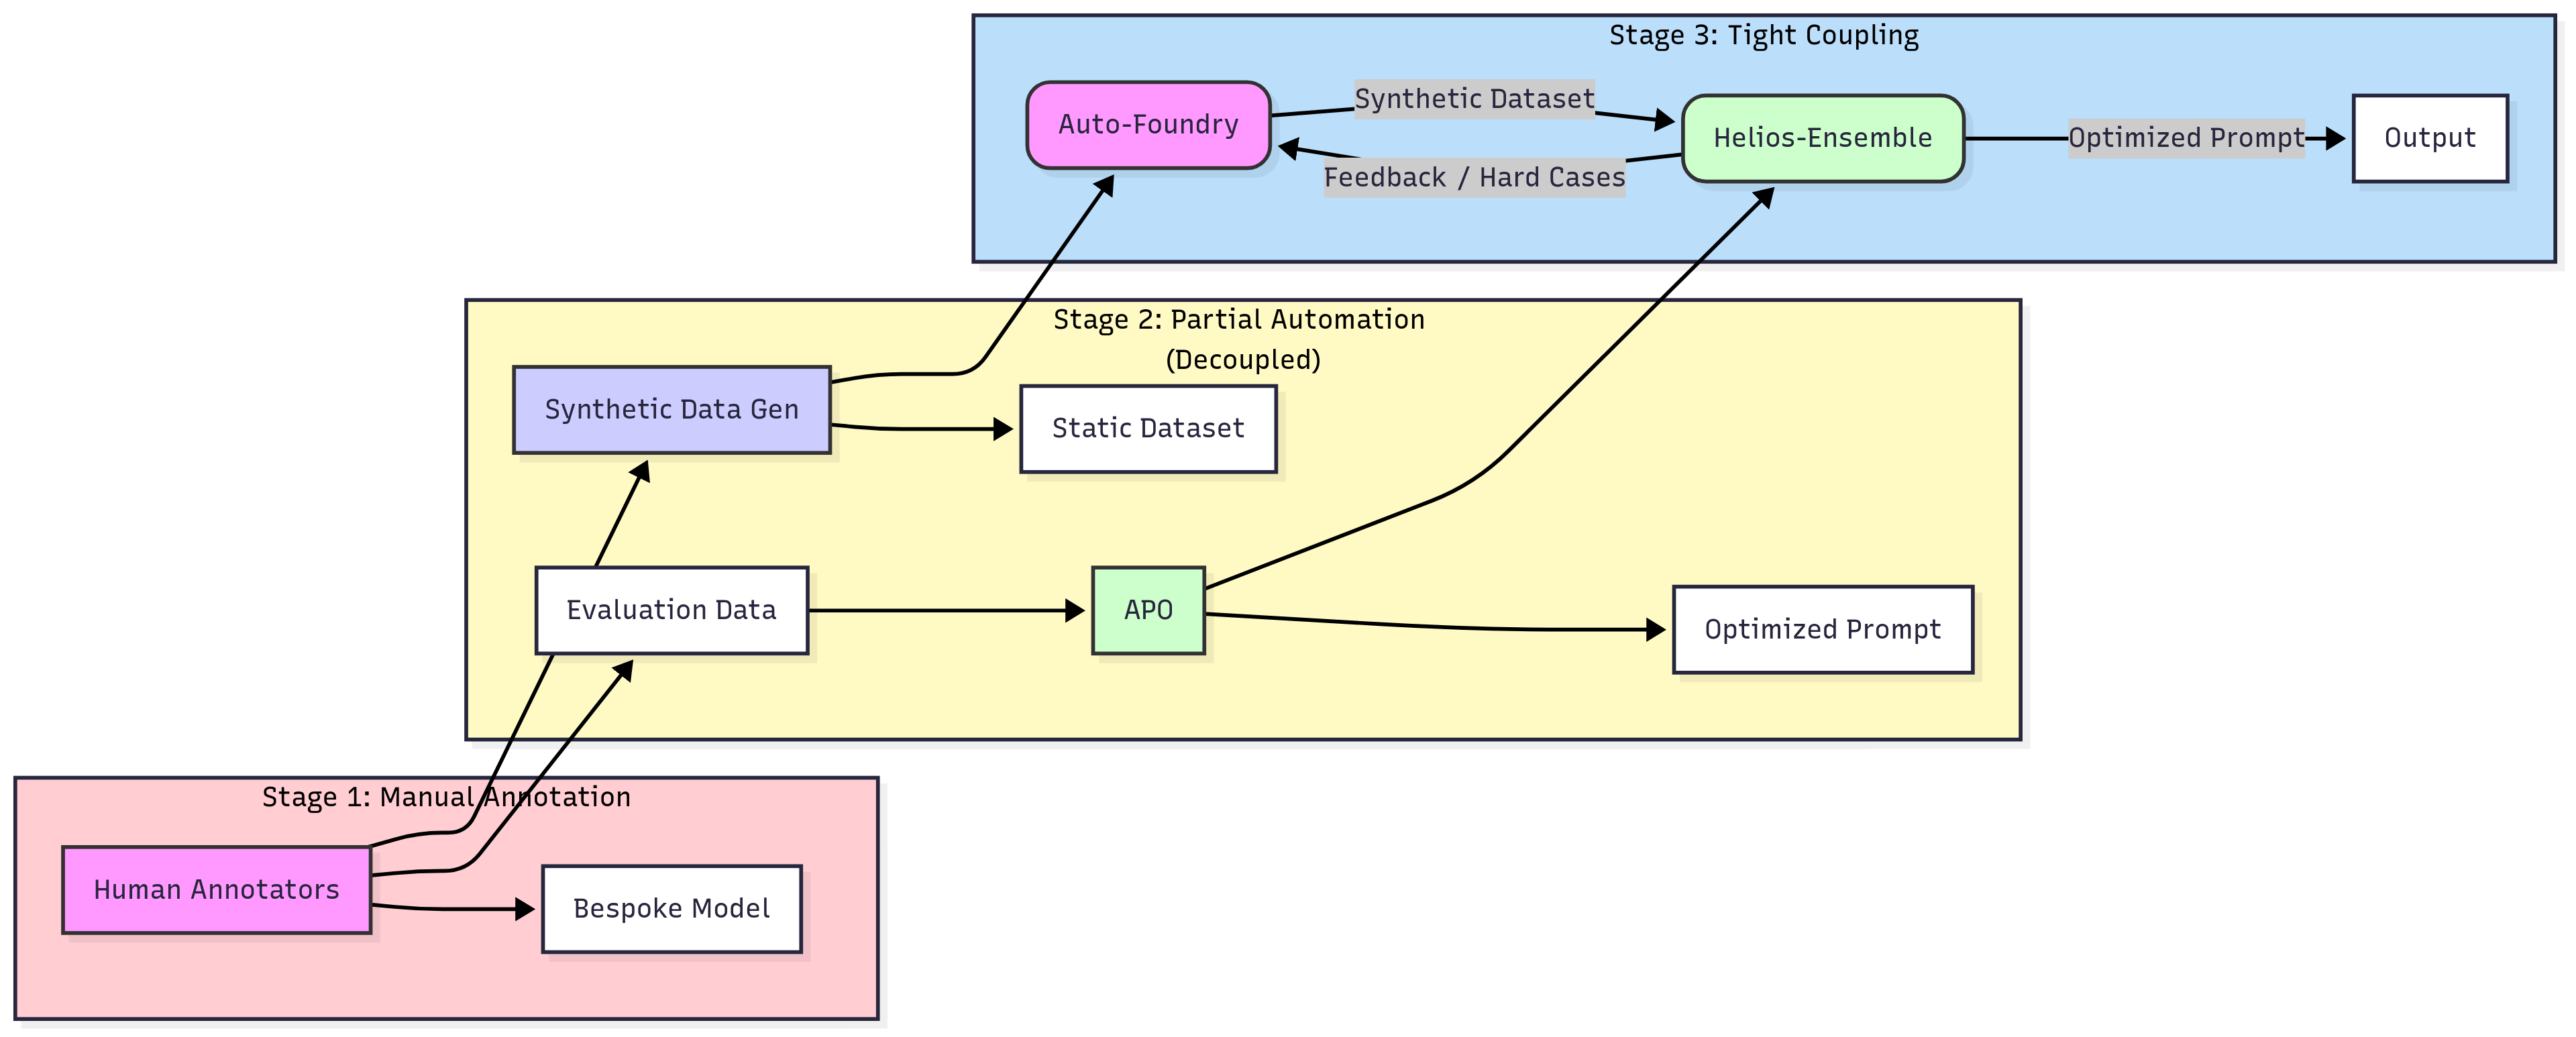
\includegraphics[width=0.9\textwidth]{evolution_timeline.png}
  \caption{Evolution of signal-extraction from manual annotation, to partial automation, to Project Helios, integrating synthetic data generation and prompt optimization in a self-improving loop.}
  \label{fig:evolution_timeline}
\end{figure}

\bigskip
\noindent\textbf{Formal Problem Statement.}
Let
\begin{itemize}[leftmargin=*,noitemsep]
  \item $\mathcal{R}$: a natural-language \emph{rubric} describing $m$ signals to be extracted;
  \item $\mathcal{C}$: an optional unlabelled corpus of $n$ text items;
  \item $\mathcal{O}$: a set of $t$ objectives with metrics  
        $\{o_1,\dots,o_t\} = \{$macro-F1, p95 latency, token cost, \ldots$\}$;
  \item $\Theta$: governance, privacy and safety constraints;
\end{itemize}
produce a set $P^{\star}$ of \emph{Pareto-optimal prompts} such that
\[
  \forall p \in P^{\star}\!:  \;
  \nexists\,p' \text{ with } 
  o_i(p') \le o_i(p)\,\forall i \text{ and } 
  o_j(p') < o_j(p)\,\text{for some } j,
\]
while satisfying $\Theta$. The optimisation budget (tokens, wall-clock) is fixed a-priori.

\section{Problem Formulation \& Key Design Decisions}
\label{sec:problem}
The previous section established the core philosophy of Helios: that tight coupling enables advanced capabilities like hard-case mining and multi-objective robustness. Realizing this vision, however, requires translating this high-level principle into a concrete set of engineering choices. This section details the nine critical design decisions that form the foundation of the Helios architecture, systematically addressing the tactical challenges of building a fully automated, closed-loop system.

\subsection*{D1: Real vs. Synthetic Data Blend \& the "Cold Start" Problem}
Real, human-annotated data offers the highest fidelity but is prohibitively expensive and slow to acquire at scale, creating a "cold start" problem for data-centric workflows. While synthetic data generated by LLMs is a cost-effective and scalable alternative, it introduces the risk of generating unrealistic or non-diverse samples that can lead to model degradation \citep{patel2024datadreamertoolsyntheticdata}.

\paragraph{Helios's Approach:} To address this, Helios adopts a hybrid, synthetic-first approach that bootstraps from a minimal set of real data (or even just the user's rubric). This addresses the cold-start problem by using a powerful "teacher" model to generate a small set of high-quality "golden" examples, which then seed a larger, more diverse synthetic dataset. This choice directly motivates the \textbf{"Blueprint"} and \textbf{"Seeding"} phases of the synthetic data generator described in Section 5, enabling rapid and affordable experimentation.

\subsection*{D2: Diversity vs. Rubric Fidelity \& Semantic Mode Collapse}
A core challenge in synthetic data generation is balancing two competing goals: ensuring every example is faithful to the user's rubric (fidelity) while also ensuring the dataset is sufficiently diverse to prevent "semantic mode collapse"—the generation of monotonous, repetitive examples that limit the model's ability to generalize \citep{yu2023largelanguagemodelattributed}.

\paragraph{Helios's Approach:} Helios addresses this by structurally separating the concerns of diversity and fidelity. The system first generates a diverse set of candidate examples using \textbf{correlated sampling}, a technique designed to introduce anti-correlation between generated instances and prevent semantic mode collapse \citep{kowshik2024corrsynthcorrelatedsampling}. Subsequently, an independent "Judge" LLM enforces rubric fidelity by filtering the candidates. This two-step process ensures the final dataset is both diverse and relevant, providing a robust foundation for the prompt optimizer.

\subsection*{D3: Single- vs. Multi-Objective Optimization \& the Hidden Trade-offs}
Signal extraction is inherently a multi-objective problem, requiring a balance between not just accuracy, but also operational metrics like latency, cost, and safety. Traditional single-objective optimization methods obscure these critical trade-offs by collapsing them into a single score, leading to "vacuum optimization" where a prompt that is optimal in a sandbox environment is brittle in production.

\paragraph{Helios's Approach:} Helios explicitly adopts a \textbf{multi-objective Pareto optimization} framework, inspired by ParetoPrompt \citep{zhao2025pareto}. This allows Helios to discover a set of \emph{Pareto-optimal} prompts that represent the best possible trade-offs between competing objectives. By presenting the user with a Pareto front of solutions, Helios enables them to select a production-ready prompt that is tailored to their specific operational constraints, such as prioritizing speed over a marginal gain in accuracy.

\subsection*{D4: Generator--Judge Independence to Mitigate Self-Reinforcement Bias}
In the synthetic data pipeline, using the same LLM to both generate and judge examples is computationally efficient but risks introducing a "self-reinforcement bias," where a model is overly lenient towards its own outputs. This can lead to a low-quality dataset that compromises the integrity of the entire optimization loop.

\paragraph{Helios's Approach:} To mitigate this, Helios enforces strict independence between the Generator and Judge LLMs. By using distinct models (or at least, distinct API endpoints with unique system prompts), we prevent information leakage and ensure that the evaluation of synthetic data is objective. This separation is critical for producing a high-quality, reliable training corpus for the downstream prompt optimizer.

\subsection*{D5: Optimizer-Guided Data Enrichment \& Overcoming Stagnation}
A static dataset, no matter how high-quality, will eventually lead to optimizer stagnation, where the prompt overfits to the training data and fails to generalize. To build robust, production-ready prompts, the system must be continuously challenged with "hard cases" that expose its weaknesses.

\paragraph{Helios's Approach:} Helios implements a closed-loop, iterative data enrichment process inspired by the principles of strategic guidance and trajectory-informed optimization \citep{wu2024stragoharnessingstrategicguidance, yang2024largelanguagemodelsoptimizers}. The prompt optimizer identifies its weakest areas (the "hard cases") and feeds this information back to the synthetic data generator. The generator then creates a new batch of targeted examples designed to address these specific weaknesses. This adaptive curriculum continuously challenges the optimizer, preventing overfitting and pushing the system towards greater generalization and reliability. This choice directly motivates the \textbf{"Hard-Case Mining"} phase in Section 5 and the \textbf{trajectory-informed context} component of the `Pareto-StraGo` algorithm in Section 6.

\subsection*{D6: Architectural Modularity to Avoid Brittleness \& Enable Evolution}
The rapid evolution of foundation models means that any monolithic system architecture is destined for obsolescence. To ensure long-term viability, the system must be designed for modularity and evolvability, allowing components to be upgraded or replaced without requiring a complete redesign.

\paragraph{Helios's Approach:} To ensure long-term viability, Helios adopts a modular, two-pillar architecture with a clear separation of concerns and well-defined interfaces, inspired by the three-layer reference architecture for FM-based systems \citep{lu2024referencearchitecturedesigningfoundation}. The core components—the Generator, Judge, and Optimizer LLMs—are designed as swappable services. This "micro-kernel-like" approach allows Helios to gracefully evolve, integrating new, more powerful foundation models as they become available and ensuring the system remains at the state-of-the-art. This also motivates the use of a \textbf{bandit-style algorithm} for dynamic strategy selection within the optimizer \citep{ashizawa2025banditbasedpromptdesignstrategy}, as it allows the system to adapt its internal optimization strategies as the underlying models change.

\subsection*{D7: Choice of Optimization Paradigm: Semantic vs. Evolutionary Search}
A fundamental decision in designing the APO pillar is the choice of optimization paradigm. \textbf{Gradient-based methods} offer efficiency but are often limited in scope. \textbf{Evolutionary algorithms} excel at broad, global exploration but can be semantically random and inefficient \citep{cui2024phaseevounifiedincontextprompt}. The \textbf{"LLM-as-Optimizer"} paradigm leverages a model's reasoning to make intelligent, targeted refinements but can be computationally intensive.

\paragraph{Helios's Approach:} Helios's `Pareto-StraGo` algorithm is a deliberate synthesis that commits to the \textbf{LLM-as-Optimizer} paradigm as its core, using strategic guidance \citep{wu2024stragoharnessingstrategicguidance} and trajectory-informed context \citep{yang2024largelanguagemodelsoptimizers} for intelligent refinement. However, it strategically incorporates concepts from evolutionary search (crossover) to escape local optima, creating a hybrid that balances intelligent, directed search with robust global exploration.

\subsection*{D8: Degree of Autonomy vs. Human-in-the-Loop Oversight}
A core operational decision is the level of system autonomy. A fully autonomous "fire-and-forget" system maximizes speed and scalability, but risks optimizing for an ambiguous rubric or getting stuck on noisy "hard cases." A system with \textbf{Human-in-the-Loop (HITL)} checkpoints, in contrast, enhances trust, safety, and robustness at the cost of speed.

\paragraph{Helios's Approach:} Helios is designed as a \textbf{primarily autonomous system} to deliver on its core value proposition of accelerating the experimental cycle from months to hours. However, its modular architecture (D6) is explicitly designed to accommodate future integration of HITL checkpoints. This allows for a flexible operational model where high-stakes or safety-critical applications can easily incorporate human oversight for tasks like rubric validation, hard-case approval, or final prompt selection from the Pareto front.

\subsection*{D9: System Statefulness and Meta-Learning Across Runs}
The final design consideration is whether the system should be \textbf{stateless} (where each run is independent) or \textbf{stateful} (where it learns from previous runs). A stateless system is simpler and guarantees that each run is an unbiased execution of the user's rubric. A stateful system, however, could achieve significant long-term efficiencies through meta-learning.

\paragraph{Helios's Approach:} The Helios framework presented in this paper is \textbf{stateless by design}. This ensures predictable, reproducible, and unbiased performance for any given signal engineering task. This choice represents a foundational step. The data-centric and modular architecture makes Helios an ideal platform for future work in stateful meta-learning, where the system could cache and reuse effective optimization strategies, prompt fragments, or synthetic data archetypes to dramatically accelerate convergence on similar tasks in the future.

\section{Project Helios Architecture (High-Level)}
\label{sec:architecture}
This section describes the high-level architecture of Project Helios, emphasizing modularity, evolvability, and responsible AI. We adopt the three-layer view from \citep{lu2024referencearchitecturedesigningfoundation}: a \textit{System Layer} (user-facing components), an \textit{Operation Layer} (core AI logic), and a \textit{Supply-Chain Layer} (foundation model sourcing). We first present a conceptual architecture diagram, then illustrate the data flow from user rubric to optimized prompt, and finally highlight key decoupling points ensuring long-term adaptability.

\begin{figure}[H]
  \centering
  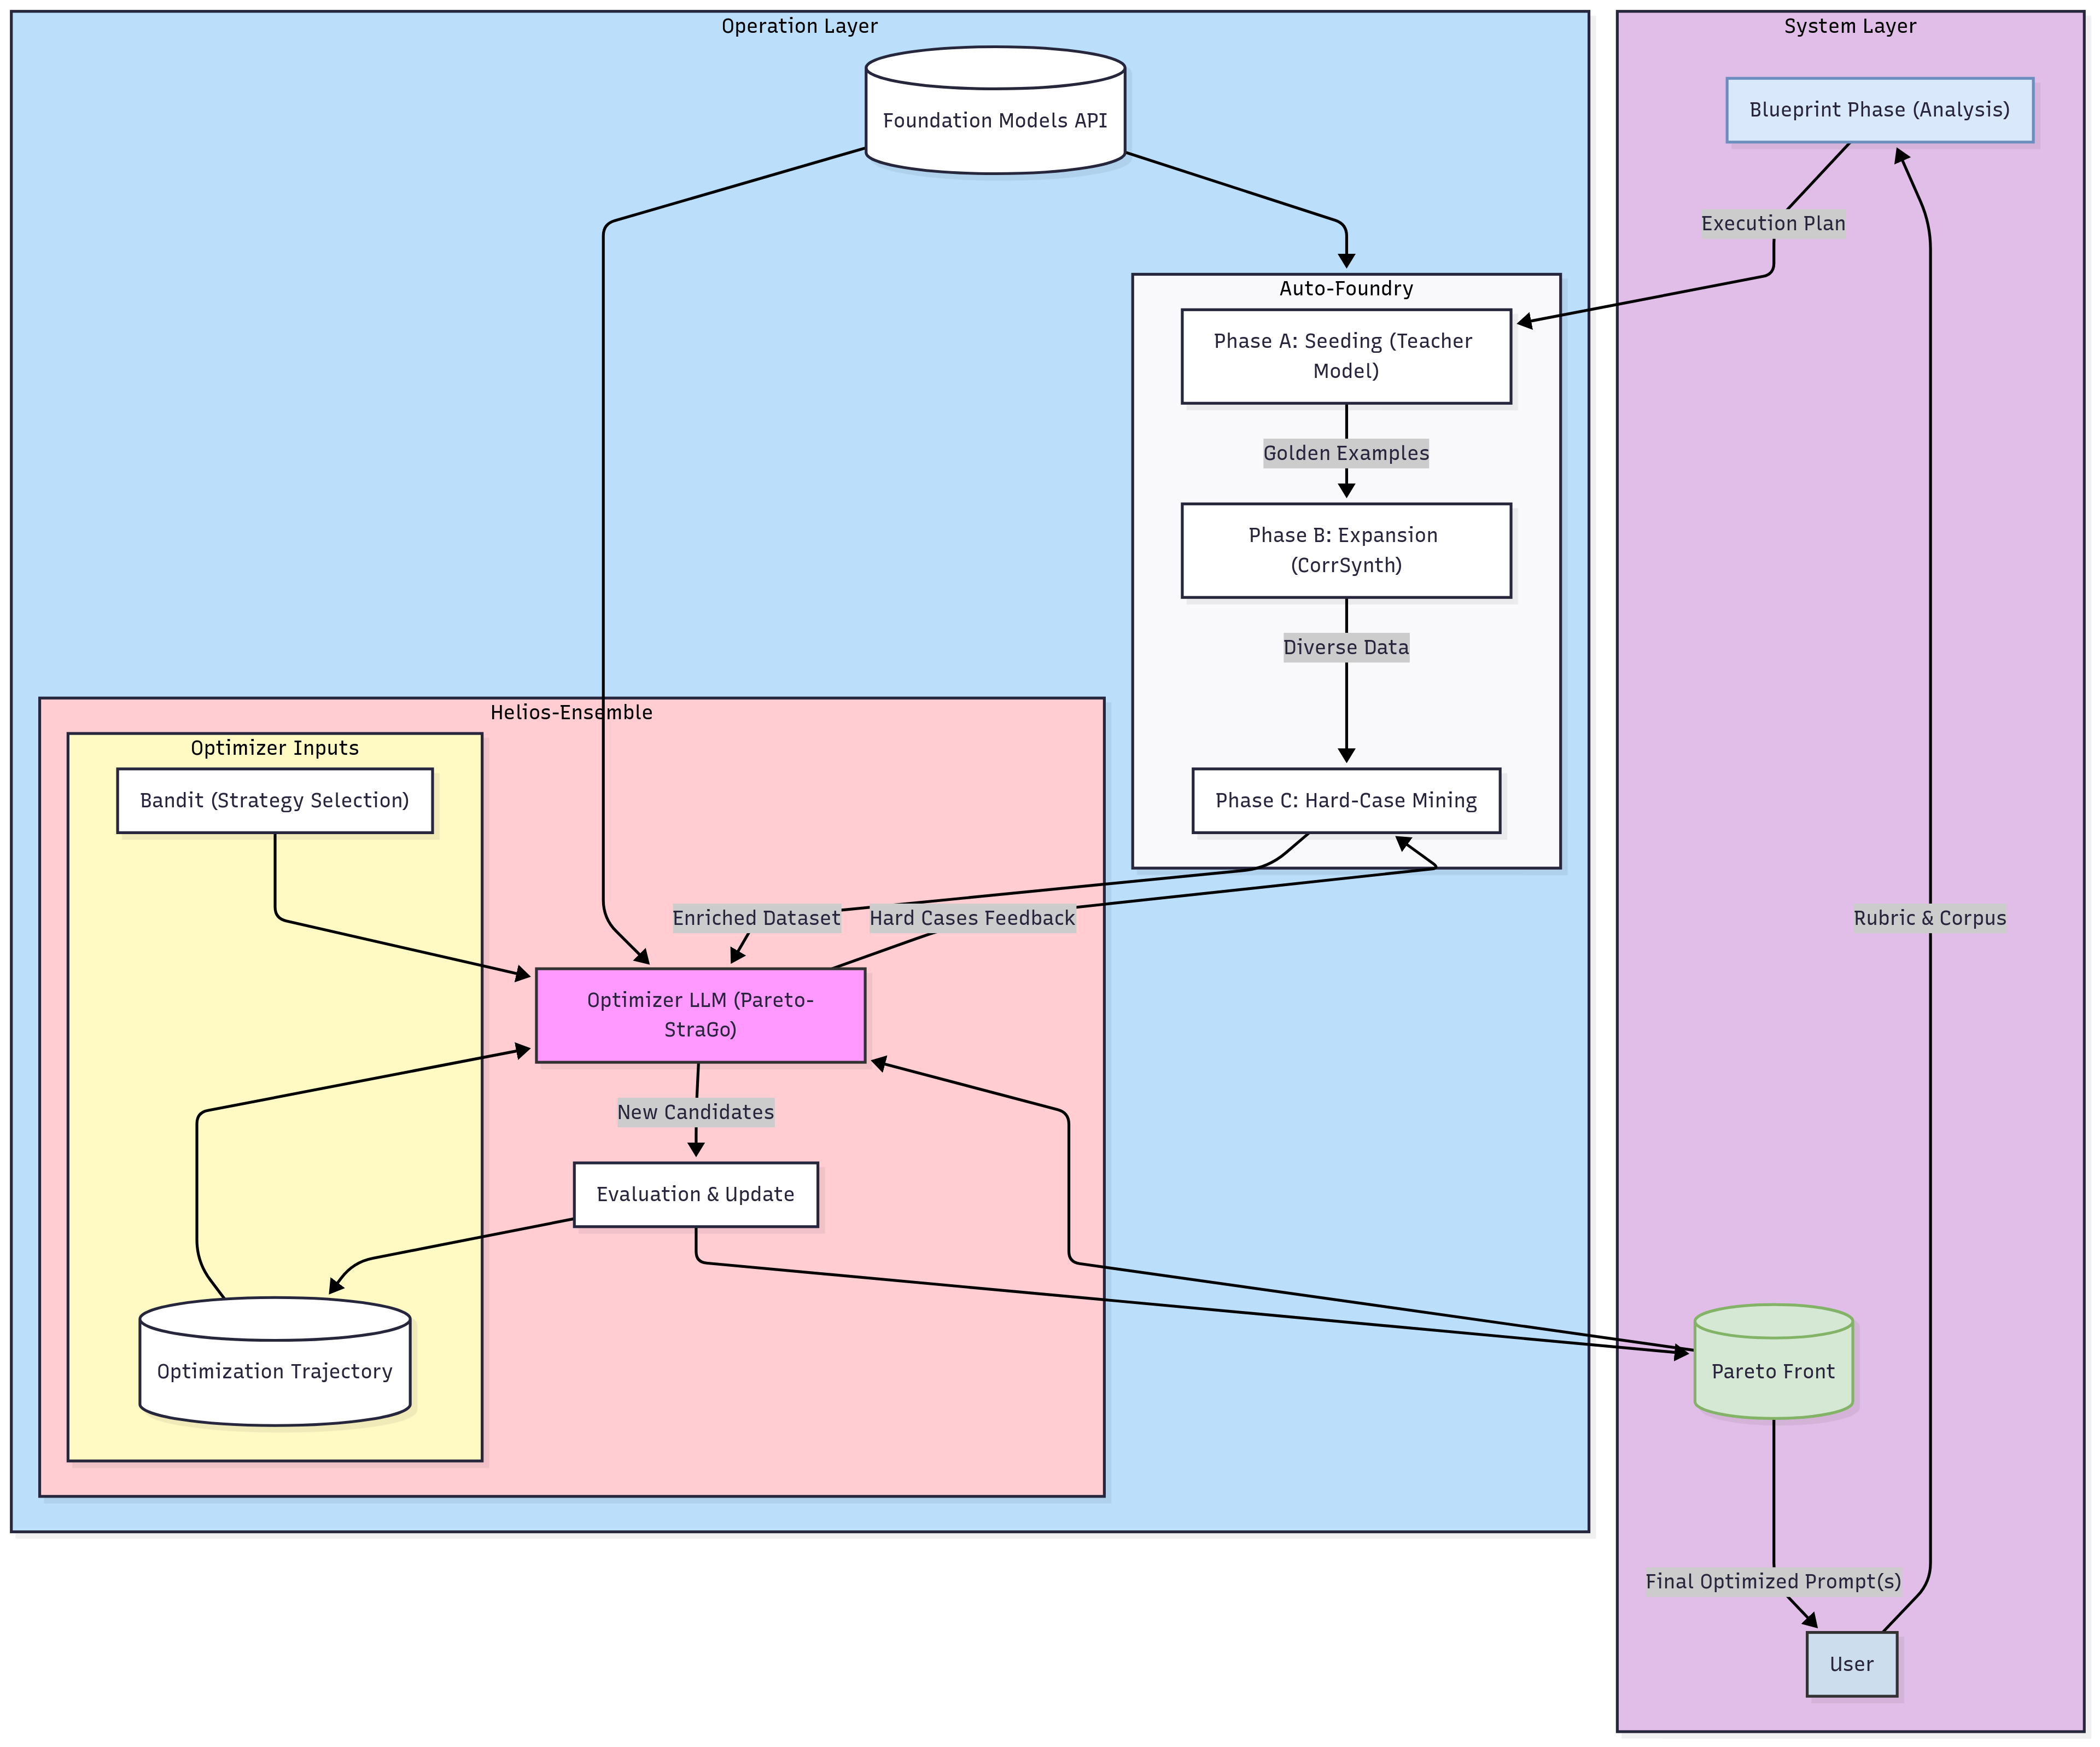
\includegraphics[width=\textwidth]{helios_architecture.png}
  \caption{The three-layer architecture of Project Helios, adapted from \cite{lu2024referencearchitecturedesigningfoundation}. The Supply-Chain Layer provides base models, the Operation Layer implements core logic, and the System Layer manages user interaction. Helios orchestrates a closed loop between the generator and optimizer to convert user rubrics into optimized prompts.}
  \label{fig:architecture}
\end{figure}

Figure~\ref{fig:architecture} shows Helios's workflow. Users provide a natural-language \textbf{rubric} and optional raw \textbf{text} corpus to the System Layer. The Operation Layer's synthetic data generator generates a synthetic dataset tailored to the rubric, using a Generator LLM (from the Supply-Chain Layer) for diverse examples and a separate Judge LLM for rubric fidelity (addressing D1, D2, D4). This dataset trains and evaluates the \textbf{APO} optimizer, which identifies Pareto-optimal prompts balancing accuracy, latency, and cost (D3). Performance metrics, especially from challenging cases, feed back into the synthetic data generator, guiding targeted data enrichment (D5). This iterative loop continues until a stable, optimized prompt emerges.

Helios's modular, micro-kernel-inspired architecture \citep{inbook} anticipates evolving foundation model capabilities. Core components—Generator, Judge, and Optimizer LLMs—are designed as swappable services with clear interfaces, enabling seamless adaptation as models mature (D6). This decoupling ensures Helios's long-term viability without fundamental redesign. Table~\ref{tab:components_vs_decisions} summarizes the mapping between architectural components and key design decisions from Section~\ref{sec:problem}.

\begin{table}[h]
  \centering
  \caption{Mapping of architectural components to key design decisions.}
  \label{tab:components_vs_decisions}
  \begin{tabular}{p{4.5cm} p{8cm}}
    \toprule
    \textbf{Architectural Component} & \textbf{Design Decision(s) Satisfied}                                                \\
    \midrule
    Synthetic Data Generator         & D1 (Data Blend \& Cold Start), D2 (Diversity Focus), D5 (Hard-Case Enrichment)       \\
    \addlinespace
    Independent Judge LLM            & D2 (Fidelity Enforcement), D4 (Generator-Judge Independence)                         \\
    \addlinespace
    Multi-Objective Optimizer        & D3 (Multi-Objective Goal), D5 (Hard-Case Identification), D7 (Optimization Paradigm) \\
    \addlinespace
    Helios System Architecture       & D6 (Modularity \& Evolvability), D8 (Autonomy vs. HITL), D9 (Statefulness)           \\
    \bottomrule
  \end{tabular}
\end{table}

\section{Pillar 1 – Zero-Config Synthetic Data}
\label{sec:autofoundry}
Helios thus automates synthetic data generation, producing diverse, rubric-aligned datasets with minimal user configuration. It employs correlated sampling for diversity, integrates feedback from the optimizer LLM for targeted hard-case mining, uses an independent judge model for quality assurance, and maintains modularity for future adaptability.

\subsection{Blueprint Phase: Automated Strategy Selection}
The synthetic data generator begins with an automated \textbf{Blueprint Phase}, analyzing user inputs to dynamically select optimal data-generation strategies. Inspired by Multi-Aspect Controllable Text Generation \citep{zhang2024lightweightmultiaspectcontrolled}, this phase includes:

\begin{itemize}[noitemsep]
  \item \textbf{Signal Complexity Analysis:} Parses the rubric to assess signal number, specificity, and correlations, guiding model and strategy selection.
  \item \textbf{Source Data Profiling:} Profiles optional source text for signal sparsity and homogeneity, informing oversampling needs.
\end{itemize}

Based on this analysis, the synthetic data generator automatically chooses the best generation strategy (e.g., few-shot or correlated sampling) and appropriate model (fast fine-tuned or powerful general-purpose), abstracting complexity from users.

\subsection{Progressive Refinement Pipeline}
After blueprinting, the synthetic data generator executes a structured three-phase pipeline inspired by modular frameworks \citep{patel2024datadreamertoolsyntheticdata} and curriculum learning:

\begin{description}[noitemsep]
  \item[Phase A (Seeding):] A powerful "teacher" model generates a small set of high-quality "golden" examples aligned with the rubric.
  \item[Phase B (Expansion \& Diversification):] Using golden examples as few-shot prompts, a faster model expands the dataset. Correlated sampling \citep{kowshik2024corrsynthcorrelatedsampling} ensures semantic diversity and prevents mode collapse.
  \item[Phase C (Hard-Case Mining):] The synthetic data generator integrates feedback from the APO, identifying challenging examples. A "critic" model selects ambiguous cases from Phase B, which the powerful teacher model uses to generate targeted, difficult examples. This adaptive curriculum, inspired by failure-case analysis \citep{wu2024stragoharnessingstrategicguidance}, enhances prompt robustness.
\end{description}

\section{Pillar 2 – Multi-Objective APO}
\label{sec:heliosensemble}

\begin{primerbox}{A Primer on Automatic Prompt Optimization (APO)}
  APO frames prompt engineering as a search problem, aiming to find instructions that maximize model performance. Key concepts include:
  \begin{itemize}[noitemsep]
    \item \textbf{Search Space:} All possible prompts (discrete text or continuous embeddings).
    \item \textbf{Optimizer:} Algorithm proposing candidate prompts (traditional or LLM-based).
    \item \textbf{Objective Function:} Metric(s) scoring prompts, either single-objective (accuracy) or multi-objective (accuracy vs. latency).
  \end{itemize}
  Helios' APO employs an optimizer LLM to explore discrete prompts under multi-objective criteria.
\end{primerbox}

Helios' APO optimizes prompts to achieve Pareto-optimality across multiple user-defined objectives. Operating on the generator's synthetic dataset, it iteratively refines candidate prompts using a novel hybrid algorithm, Pareto-StraGo. This section describes the ensemble's conceptual foundations, core optimization algorithm, and strategy selection approach.

The computational complexity of Helios' APO is dominated by prompt evaluation. For a population of $N$ prompts, dataset of $K$ examples, and $T$ objectives, each iteration has complexity $O(N \cdot K \cdot T \cdot C_{LLM})$, where $C_{LLM}$ is the cost per LLM inference. Bandit-based strategy selection and prompt generation have comparatively negligible complexity.

\subsection{Conceptual Foundation: Optimizer LLM}
Helios' APO leverages Large Language Models as optimizers \citep{yang2024largelanguagemodelsoptimizers}, replacing traditional numerical methods with LLM-driven optimization guided by a meta-prompt. This meta-prompt includes candidate prompts, multi-objective performance scores (e.g., accuracy, latency), and strategic instructions. The optimizer LLM analyzes this information to iteratively propose improved prompts, utilizing its semantic reasoning capabilities for non-gradient-based optimization.

\subsection{Pareto-StraGo: A Hybrid Optimization Algorithm}
The APO employs a novel hybrid algorithm synthesizing four state-of-the-art prompt optimization techniques we call Pareto-StraGo:

\begin{itemize}
  \item \textbf{Pareto Optimization (from ParetoPrompt):} To handle the inherent multi-objective nature of signal extraction, ParetoPrompt maintains a Pareto front of prompts, explicitly balancing trade-offs among objectives like accuracy and cost \citep{zhao2025pareto}.
  \item \textbf{Strategic Guidance:} As per the work in StraGo, the optimizer analyzes successes and failures to generate targeted improvement strategies, enhancing refinement beyond trial-and-error \citep{wu2024stragoharnessingstrategicguidance}.
  \item \textbf{Evolutionary Crossover (from PhaseEvo):} To escape local optima and encourage innovation, we propose the combining of high-performing prompts to create novel candidates, promoting diversity and avoiding local optima \citep{cui2024phaseevounifiedincontextprompt}.
  \item \textbf{Trajectory-Informed Context (from OPRO):} Includes historical optimization trajectories in the meta-prompt, enabling informed, pattern-aware prompt proposals \citep{yang2024largelanguagemodelsoptimizers}.
\end{itemize}

This integrated approach ensures efficient, innovative, and directed optimization compared to single-method paradigms.

\begin{table}[h]
  \centering
  \caption{Notation used}
  \label{tab:notation}
  \begin{tabular}{cl}
    \toprule
    \textbf{Symbol}       & \textbf{Description}                \\
    \midrule
    $G$                   & The Generator LLM                   \\
    $J$                   & The Judge LLM                       \\
    $O$                   & The Optimizer LLM                   \\
    $\mathcal{R}$         & User-provided signal rubric         \\
    $\mathcal{D}_{synth}$ & The generated synthetic dataset     \\
    $\mathcal{P}$         & The population of candidate prompts \\
    $p^*$                 & A Pareto-optimal prompt             \\
    \bottomrule
  \end{tabular}
\end{table}

\begin{algorithm}[H]
  \caption{Pareto-StraGo Optimization Loop (Conceptual)}
  \label{alg:paretostrago}
  \SetAlgoLined
  \KwIn{Initial prompt population $P_0$, Objective functions $O$, Strategy set $S$, Population size $k$}
  \KwOut{Pareto-optimal prompt set $P^*$}
  $P \leftarrow P_0$\;
  \While{not converged}{
    Evaluate each prompt $p \in P$ on objectives $O$ to get scores\;
    Update Pareto front $P^*$ with non-dominated prompts from $P$\;
    Select strategy $s \in S$ using bandit algorithm\;
    Construct meta-prompt with $P^*$, scores, and strategy $s$\;
    Generate new candidate prompts $P_{new}$ using Optimizer LLM\;
    $P \leftarrow \text{CullToSize}(P \cup P_{new}, k)$\;
  }
\end{algorithm}

\subsection{Bandit-Style Strategy Selection and Feasibility}
Helios' APO employs the bandit-style algorithm from \cite{ashizawa2025banditbasedpromptdesignstrategy} to select the most effective improvement strategy (e.g., "rephrase," "add example," "simplify") at each optimization step. Strategies are treated as arms of a multi-armed bandit, dynamically allocating budget to balance exploration of new strategies and exploitation of proven ones, optimizing improvements on the Pareto front.

The primary computational cost—evaluating candidate prompts against the synthetic dataset—is parallelizable, as prompts are independently assessed. Prompt generation by the optimizer LLM is sequential but constitutes a minor fraction of total compute time. This architecture ensures scalability and practical feasibility, efficiently exploring a vast prompt space for high-performing, multi-objective solutions. In contrast, earlier methods like AutoPrompt \citep{shin2020autopromptelicitingknowledgelanguage}, DSPy's MIPRO \citep{opsahlong2024optimizinginstructionsdemonstrationsmultistage}, or soft-prompt tuning \citep{lester2021powerscaleparameterefficientprompt} often rely on single-objective functions and less efficient search strategies.

\section{Feasibility \& Illustrative Scenarios}
\label{sec:feasibility}
This paper proposes a conceptual architecture for Project Helios without a full experimental implementation. To demonstrate feasibility, we present structured analyses and thought experiments. First, we compare the Helios pipeline's costs and benefits against traditional manual methods. Next, we illustrate the system's end-to-end operation through a hypothetical scenario. Finally, we map key technical and ethical risks to mitigating features within Helios, highlighting its robustness and viability.

\subsection{Cost--Benefit Analysis}
\label{subsec:cost_benefit}
We assess Helios's economic viability by comparing it to a traditional manual signal-extraction pipeline. Manual methods incur high recurring labor costs for data annotation, whereas Helios involves higher initial computational costs amortized over time. As shown in Table~\ref{tab:cost_benefit}, Helios primarily saves costs by automating data generation and prompt optimization—the most expensive and time-consuming manual phases. Helios's cost sensitivity depends mainly on corpus size and the number of extracted signals, following scaling laws of foundation models \citep{kaplan2020scalinglawsneurallanguage}.

\begin{table}[h]
  \centering
  \caption{Illustrative Cost-Benefit Analysis Based on Token Consumption}
  \label{tab:cost_benefit}
  \begin{tabular}{p{3.5cm} p{4.5cm} p{4.5cm}}
    \toprule
    \textbf{Phase}              & \textbf{Manual Pipeline Cost (Illustrative)} & \textbf{Helios Pipeline Cost (Illustrative)}                   \\
    \midrule
    \textbf{Data Generation}    & \$10,000 (e.g., 2,000 annotations @ \$5/ea)  & \$1,500 (10k examples, ~300M tokens @ \$5/M tokens for GPT-4o) \\
    \textbf{Optimization}       & \$5,000 (Engineer time for fine-tuning)      & \$500 (100 prompt candidates, 10 iterations, ~100M tokens)     \\
    \midrule
    \textbf{Total (per signal)} & \textbf{\$15,000 (Recurring)}                & \textbf{\$2,000 (Amortized Compute)}                           \\
    \bottomrule
  \end{tabular}
  \caption*{Note: Token counts and costs are illustrative, assuming a 10k-example synthetic dataset and a moderately complex optimization run. Actual costs depend on corpus size, signal complexity, and the chosen foundation models.}
\end{table}

\subsection{Walk-Through Example: "Consequence Awareness" Signal}
\label{subsec:walkthrough}
To illustrate Helios concretely, consider a hypothetical scenario: a sales organization aims to extract a "consequence awareness" signal from sales call transcripts, identifying when salespeople highlight negative impacts of customer inaction.

\begin{enumerate}
  \item \textbf{User Input:} User provides rubric: ``Identify sentences where the salesperson explains negative business impacts of not adopting our solution.''
  \item \textbf{Initial Data Generation:} Generator LLM ($G$) creates diverse examples based on the rubric; Judge LLM ($J$) filters for quality.
        \begin{itemize}
          \item \textit{Synthetic Positive:} ``Without our security patch, a data breach could lead to regulatory fines exceeding \$1M.''
          \item \textit{Synthetic Negative:} ``Our solution offers best-in-class performance and a user-friendly interface.''
        \end{itemize}
  \item \textbf{Initial Optimization:} Optimizer LLM ($O$) uses this dataset to find an initial prompt, e.g., \texttt{Does the sentence describe a negative outcome?}
  \item \textbf{Hard-Case Identification:} This prompt fails on a subtle evaluation case:
        \begin{itemize}
          \item \textit{Hard Case:} ``Your team's workflow velocity will likely drop by another 15\% next quarter if the tool integration isn't addressed.'' (Correct: Yes, Predicted: No).
        \end{itemize}
  \item \textbf{Feedback Loop to the Synthetic Data Generator:} Optimizer flags this failure. $G$ generates additional examples of \textit{implied} negative consequences, e.g., ``Sticking with your legacy system means engineers continue spending 10 hours weekly on manual patching.''
  \item \textbf{Final Prompt Optimization:} Using enriched data, $O$ finds a robust, Pareto-optimal prompt: ``\texttt{Analyze the text. Does it state or imply a negative business consequence from inaction? Answer Yes or No.}''
\end{enumerate}

This example demonstrates Helios's self-improving pipeline, progressing from a simple rubric to a nuanced, production-ready prompt.

\subsection{Comparative Thought Experiment}
\label{subsec:comparative_thought_experiment}
We now examine how partial-automation ("Stage 2") alternatives handle the "consequence awareness" scenario:

\begin{itemize}
  \item \textbf{Alternative A (Synthetic Data Only):} A synthetic-data-only system (e.g., \citep{patel2024datadreamertoolsyntheticdata}) generates datasets from the initial rubric but lacks optimizer feedback, missing subtle, challenging examples. A human engineer would likely produce the initial flawed prompt, unaware of weaknesses with implied consequences.

  \item \textbf{Alternative B (APO Only):} A prompt-optimizer-only system (e.g., \citep{pryzant2023automaticpromptoptimizationgradient}) trained on limited, fixed data might yield a prompt effective only for that dataset. Without broader data coverage, it would fail to generalize to unseen, subtle cases surfaced by Helios's hard-case mining.
\end{itemize}

This comparison highlights Helios's advantage: tightly integrating data generation and optimization addresses partial-automation limitations, enabling robust, generalizable signal extraction.

\subsection{Risk \& Mitigation Mapping}
\label{subsec:risk_mitigation}
Any complex AI system introduces potential risks. The Helios architecture incorporates several features designed to mitigate these risks proactively. Table~\ref{tab:risk_mitigation} maps the primary risk categories to their corresponding mitigation features within Helios.

\begin{table}[h]
  \centering
  \caption{Risk and Mitigation Mapping in the Helios Architecture.}
  \label{tab:risk_mitigation}
  \begin{tabular}{p{2.5cm}p{4.5cm}p{5cm}}
    \toprule
    \textbf{Risk Category} & \textbf{Specific Risk}                                                                                            & \textbf{Helios Mitigation Feature}                                                                                                                      \\
    \midrule
    Technical              & Mode collapse in data generator, leading to low-diversity data.                                                   & Correlated sampling in generator to ensure breadth of examples.                                                                                         \\
                           & Optimizer overfits to "easy" data and fails to generalize.                                                        & Closed-loop hard-case mining forces the optimizer LLM to confront its weaknesses.                                                                       \\
    \midrule
    Ethical                & Synthetic data amplifies societal biases present in the source corpus \citep{yu2023largelanguagemodelattributed}. & Independent Judge LLM can be tasked with enforcing fairness constraints defined in the rubric.                                                          \\
                           & Generated signals are used for malicious or unfair purposes.                                                      & Guardrails and multi-aspect controlled generation techniques \citep{zhang2024lightweightmultiaspectcontrolled} can be integrated into the Judge module. \\
    \midrule
    Operational            & High compute cost of generation and optimization makes the system impractical.                                    & Modular architecture (D6) allows for swapping in smaller, more efficient models. Cost is amortized over the signal's lifecycle.                         \\
                           & System becomes obsolete as foundation models evolve.                                                              & Micro-kernel design with well-defined interfaces allows for graceful evolution and component replacement.                                               \\
    \bottomrule
  \end{tabular}
\end{table}

\section{Discussion}
\label{sec:discussion}
This paper has articulated a conceptual architecture for Project Helios, a system designed to automate predictive signal extraction by tightly coupling synthetic data generation with multi-objective prompt optimization. In this section, we step back to discuss the broader implications of this framework. We examine its strategic value for enterprises, acknowledge its inherent limitations and ethical considerations, and outline a pragmatic roadmap for its implementation.

\subsection{Strategic Value for Enterprises}
The primary strategic value of Project Helios lies in its potential to significantly alter the economics and velocity of signal engineering within an enterprise. The current manual paradigm is slow and expensive, creating a bottleneck that forces teams to be highly selective about which predictive signals they can afford to explore. Helios is designed to dismantle this bottleneck. By automating the most labor-intensive parts of the workflow—data annotation and prompt engineering—the framework can reduce the cycle time for signal development from months to hours. This acceleration enables a much broader, more exploratory approach to feature engineering. Teams can test a vast combinatorial space of potential signals from their unstructured text data, leading to the discovery of novel, high-value predictors that would have been infeasible to investigate manually. This capability translates directly into more accurate forecasts, better-informed business decisions, and a significant competitive advantage.

\subsection{Limitations}
Despite its potential, the proposed Helios architecture has several important limitations that warrant discussion.
\begin{itemize}
  \item \textbf{Dependence on Rubric Quality:} The entire Helios pipeline is initiated by a user-provided rubric. The quality of the final, optimized prompt is therefore capped by the clarity and correctness of this initial definition. A vague, ambiguous, or poorly formulated rubric will inevitably lead to the generation of a suboptimal or irrelevant signal.
  \item \textbf{Compute Costs:} While we argue that Helios is more cost-effective than manual annotation in the long run, the initial compute cost for generating and optimizing on a large synthetic dataset is non-trivial. The token consumption required for the synthetic data generator and APO pillars could present a significant upfront investment, potentially posing a barrier for organizations with limited computational budgets.
  \item \textbf{Synthetic Data Realism:} Although techniques like correlated sampling and hard-case mining are employed to enhance data quality, a gap will always exist between synthetic and real-world data. The generated dataset may fail to capture the full spectrum of linguistic nuance, domain-specific jargon, or rare events present in the true data distribution, a well-documented challenge in the field \citep{nadas2025syntheticdatagenerationusing}.
\end{itemize}

\subsection{Ethical Considerations}
The automation of signal extraction introduces significant ethical considerations that must be addressed by design. The most pressing of these is the risk of \textbf{bias amplification}. Foundation models trained on broad internet data can inherit and perpetuate societal biases related to gender, race, and other protected attributes \citep{yu2023largelanguagemodelattributed}. The synthetic data generator could inadvertently concentrate these biases in the synthetic dataset, leading to the creation of unfair or discriminatory signals. The primary mitigation for this risk lies in the independent Judge LLM, which can be tasked with enforcing fairness constraints and filtering out biased content.\footnote{The effectiveness of using an LLM as a fairness auditor is an active area of research and a key assumption in our proposed architecture.}

Furthermore, the power to rapidly generate predictive signals carries a risk of \textbf{misuse}. For example, the system could be used to create signals that identify and target vulnerable populations for predatory purposes. To counter this, the Helios architecture must incorporate robust safety guardrails. Techniques for multi-aspect attribute control \citep{zhang2024lightweightmultiaspectcontrolled, yu2024controlledtextgenerationblackbox} can be integrated into the Judge module to provide explicit guardrails against generating undesirable or harmful signals.

\subsection{Implementation Roadmap}
\label{subsec:implementation_roadmap}
We envision the development of Project Helios as a staged initiative, beginning with a minimal viable product (MVP) and scaling towards a full-featured enterprise platform.

\begin{itemize}
  \item \textbf{Phase 1: MVP and Pilot Program.} The initial phase would build a proof-of-concept. The MVP would implement the core feedback loop between the and optimizer for a single-objective optimization task. We would then partner with one or two internal teams to pilot the system on real-world forecasting problems, gathering baseline performance data and user feedback.
  \item \textbf{Phase 2: Generalization and Multi-Objective Expansion.} Based on the pilot's success, the second phase would focus on generalizing the framework. This includes implementing the full multi-objective capabilities of Pareto-StraGo and expanding the library of strategic guidance prompts. The goal of this phase is to create a robust, configurable platform that can serve a wider range of signal extraction tasks.
  \item \textbf{Phase 3: Enterprise-Wide Roll-out.} The final phase would involve deploying Helios as an internal platform for general use. This would require developing a user-friendly interface for rubric definition and objective selection, as well as comprehensive documentation and support. The long-term vision is to establish Helios as a central, central tool for data-driven decision-making across the enterprise.
\end{itemize}

\section{Conclusion \& Future Work}
\label{sec:conclusion}
This paper has introduced Project Helios, a conceptual architecture designed to automate the extraction of predictive signals from unstructured text. We have argued that the key to unlocking this capability lies in the tight coupling of two advancing fields: synthetic data generation and automatic prompt optimization. The proposed two-pillar architecture, featuring a zero-config synthetic data generator and multi-objective prompt optimizer, provides a pattern-oriented framework for building a system that can significantly accelerate the signal engineering lifecycle. By formalizing the problem, mapping out key design decisions, and grounding the architecture in established software engineering principles, we have laid the groundwork for a new class of automated, self-improving signal extraction systems.

The immediate next step for Project Helios is to build a minimal proof-of-concept, as outlined in our implementation roadmap (Section~\ref{subsec:implementation_roadmap}). The initial focus will be on validating the core feedback loop between the data generator and a single-objective prompt optimizer with a small set of pilot partners. This will allow us to gather empirical data on the system's performance and refine its core algorithms.

Looking further ahead, the long-term vision for Helios extends beyond textual signals. The modular architecture is designed to accommodate multimodal inputs, allowing for the extraction of predictive signals from images, audio, and other data sources. We also envision a future where the optimization process becomes fully adaptive and real-time, with the APO continuously refining prompts based on live production data. Ultimately, we see Project Helios not as a standalone system, but as a critical component in a larger ecosystem of foundation-model-powered agents, providing the essential capability of transforming raw, unstructured information into actionable, predictive intelligence.

\newpage
\bibliographystyle{plainnat}
\bibliography{edictive-arch}

\newpage
\appendix
\section{Glossary of Key Terms}
\begin{description}
  \item[Rubric] A set of natural-language rules provided by a user that defines the criteria for a predictive signal.
  \item[Correlated Sampling] A synthetic data generation technique that prompts an LLM to produce a portfolio of related but varied examples simultaneously to enhance diversity.
  \item[Hard-Case Mining] The process of identifying examples where a model performs poorly and using them to guide further training or data generation.
  \item[Pareto Front] In multi-objective optimization, the set of all solutions for which no objective can be improved without degrading at least one other objective.
  \item[Bandit Algorithm] A class of algorithms for sequential decision-making that balances exploring new options with exploiting known good options.
\end{description}

\section{Related Work}
\label{sec:relatedwork}
This section situates Project Helios within the context of several related fields. We first review the landscape of synthetic data generation and automatic prompt optimization, the two core technologies that Helios integrates. We then briefly touch upon classic prompt design techniques and the broader field of time-series foundation models to clarify Helios's unique contribution. Finally, we ground our architectural choices in established software engineering patterns.

\subsection{Synthetic Data Generation}
The use of generative models to create synthetic training data is a well-established technique for overcoming data scarcity. Early approaches in natural language processing, such as back-translation for neural machine translation \citep{sennrich2016improvingneuralmachinetranslation}, demonstrated the value of artificially generated data. The advent of LLMs has dramatically expanded the possibilities, enabling the generation of high-quality, human-like text for a wide range of tasks \citep{nadas2025syntheticdatagenerationusing}. Modern frameworks like DataDreamer \citep{patel2024datadreamertoolsyntheticdata} have begun to standardize these workflows. However, a central challenge remains: ensuring the quality and diversity of the generated data. Research has shown that naive generation can lead to significant attribute bias and a lack of diversity \citep{yu2023largelanguagemodelattributed}, or fail to satisfy complex logical constraints \citep{fedoseev2024constraint}. Helios's generation pillar directly addresses these challenges by incorporating techniques for diversity \citep{kowshik2024corrsynthcorrelatedsampling} and using an independent judge to enforce rubric fidelity.

\subsection{Automatic Prompt Optimization (APO)}
Automatic Prompt Optimization (APO) seeks to automate the discovery of the most effective natural language instructions to guide LLMs. The field has evolved rapidly, moving from gradient-based methods that tune continuous soft prompts \citep{lester2021powerscaleparameterefficientprompt} to discrete search techniques that edit textual prompts directly \citep{pryzant2023automaticpromptoptimizationgradient}. A comprehensive survey of heuristic-based search methods can be found in \citep{cui2025automaticpromptoptimizationheuristic}. A particularly powerful paradigm is the concept of using an LLM as the optimizer LLM itself \citep{yang2024largelanguagemodelsoptimizers}. Recent work in this area has focused on developing more sophisticated search strategies, including multi-objective approaches that find Pareto-optimal prompts \citep{zhao2025pareto}, the use of strategic guidance to make the optimization process more directed \citep{wu2024stragoharnessingstrategicguidance}, and bandit-style algorithms for efficient strategy selection \citep{ashizawa2025banditbasedpromptdesignstrategy}. The APO pillar builds directly on these advances, proposing a novel hybrid algorithm, Pareto-StraGo, that synthesizes these state-of-the-art techniques.

\subsection{Classic Prompt Design Techniques}
The field of APO builds upon a foundation of classic prompt engineering techniques. Early work like AutoPrompt \citep{shin2020autopromptelicitingknowledgelanguage} demonstrated that discrete prompts could be automatically generated to elicit specific knowledge from language models. Concurrently, methods like prompt tuning \citep{lester2021powerscaleparameterefficientprompt} showed that lightweight, continuous "soft prompts" could be learned to adapt frozen LLMs to new tasks with remarkable parameter efficiency. Manual techniques, most notably chain-of-thought prompting \citep{wei2023chainofthoughtpromptingelicitsreasoning}, revealed that structuring a prompt to elicit intermediate reasoning steps could significantly improve performance on complex tasks. Project Helios automates and extends these foundational ideas, using an optimizer to discover complex prompt structures that go beyond simple instruction-following.

\subsection{Time-Series Foundation Models}
Project Helios is situated within the broader research program of building foundation models for time-series analysis. A growing body of work is focused on developing large, pre-trained models that can perform zero-shot forecasting across a wide range of domains \citep{ansari2024chronoslearninglanguagetime, das2024decoderonlyfoundationmodeltimeseries}. These models often leverage textual information to improve their predictions, using techniques like reprogramming LLMs \citep{jin2024timellmtimeseriesforecasting} or developing autoregressive forecasters that can process natural language context \citep{liu2024autotimesautoregressivetimeseries}. Other work has focused on building large-scale, multi-domain models from the ground up \citep{xiao2025timefoundfoundationmodeltime, shi2025timemoebillionscaletimeseries}. While these models are designed to \textit{consume} textual signals, Helios addresses the critical antecedent problem of \textit{producing} them from raw, unstructured text. The Helios framework can be viewed as an essential upstream component in an end-to-end forecasting pipeline, generating the high-quality, contextual features that models like Time-LLM or Chronos require to achieve state-of-the-art performance.

\subsection{Architectural Pattern References}
The design of Project Helios is not ad-hoc but is grounded in established principles of software architecture. The system's modular, two-pillar structure is an application of the micro-kernel pattern, which emphasizes building a system around a minimal core of functionality and treating other components as pluggable extensions \citep{inbook}. This architectural choice is motivated by the need for evolvability in the rapidly changing foundation model landscape. Furthermore, our high-level architectural view, which separates the system into Supply-Chain, Operation, and System layers, is directly adapted from the reference architecture for foundation-model-based systems proposed by \citep{lu2024referencearchitecturedesigningfoundation}. Adopting these established patterns provides a robust and principled foundation for the Helios framework.

\end{document}

